\section{Challenges and Future}
\makesubcontentsslides

\subsection{Challenges}

\begin{frame}
  \begin{block}{Challenges}
    \begin{itemize}[<+-|alert@+>]
      \item Perceptions.\\
      ``\emph{R?  Isn't that slow?}'' -- HPC people\\
      ``\emph{HPC?  Isn't that hard?}'' -- R people
      \item Bringing R community to large platforms
      \item Distributed data input
      \item Bringing interactivity back
      \item Performance dependence on data layout
    \end{itemize}
  \end{block}
\end{frame}

\begin{frame}
  \begin{block}{Covariance Revisited: Data layout parameter calibration}
    \begin{center}
     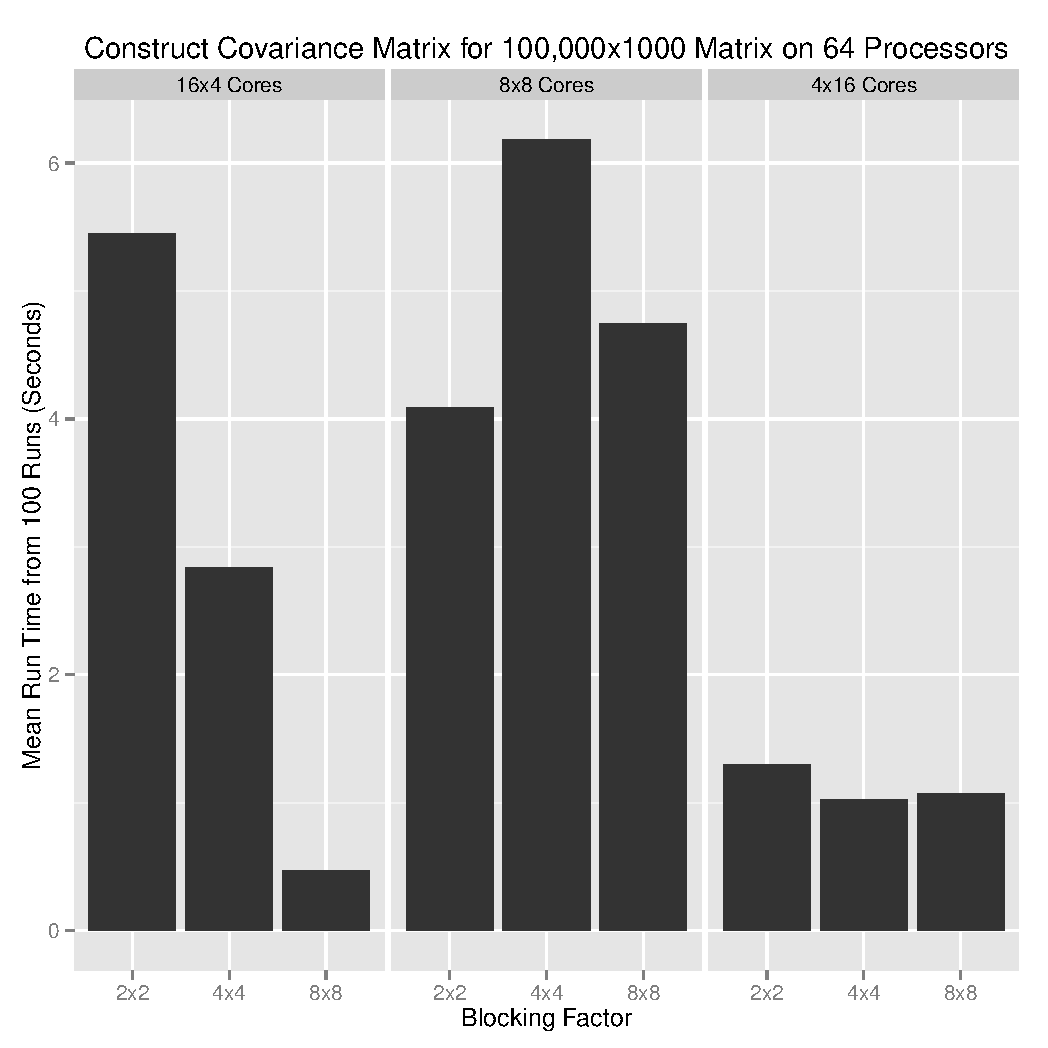
\includegraphics[width=10cm, height=7cm]{../common/pics/cov_param}
    \end{center}
  \end{block}
\end{frame}

\subsection{Future Work}

\begin{frame}
  \begin{block}{Future Work}
  \begin{itemize}
    \item Starting a 3 year NSF grant to
      \begin{itemize}
      \item Bring back interactivity via client/server
      \item Simplify parallel data input
      \item Begin DPLASMA integration
      \end{itemize}
    \item Optimization for heterogeneous architectures
    \item In-situ use with simulations
  \end{itemize}
  \end{block}
\end{frame}

\begin{frame}
  \begin{block}{Batch and Interactive. What is the difference?}
    \begin{itemize}
    \item High-level functional language: a function is a ``batch'' script
    \item \R ``An interactive environment to use batch scripts''
    \item Current \pbdR for ``batch/server'' big platforms
    \item Client under development
      \begin{itemize}
      \item Bridge laptop to login node to resource manager to cluster
      \item Relationship of big data (server side) to little data (client side)
      \end{itemize}
    \item Intuitive parallel data input under development
    \end{itemize}
  \end{block}
\end{frame}

\begin{frame}{Cluster/Supercomputer Environment}
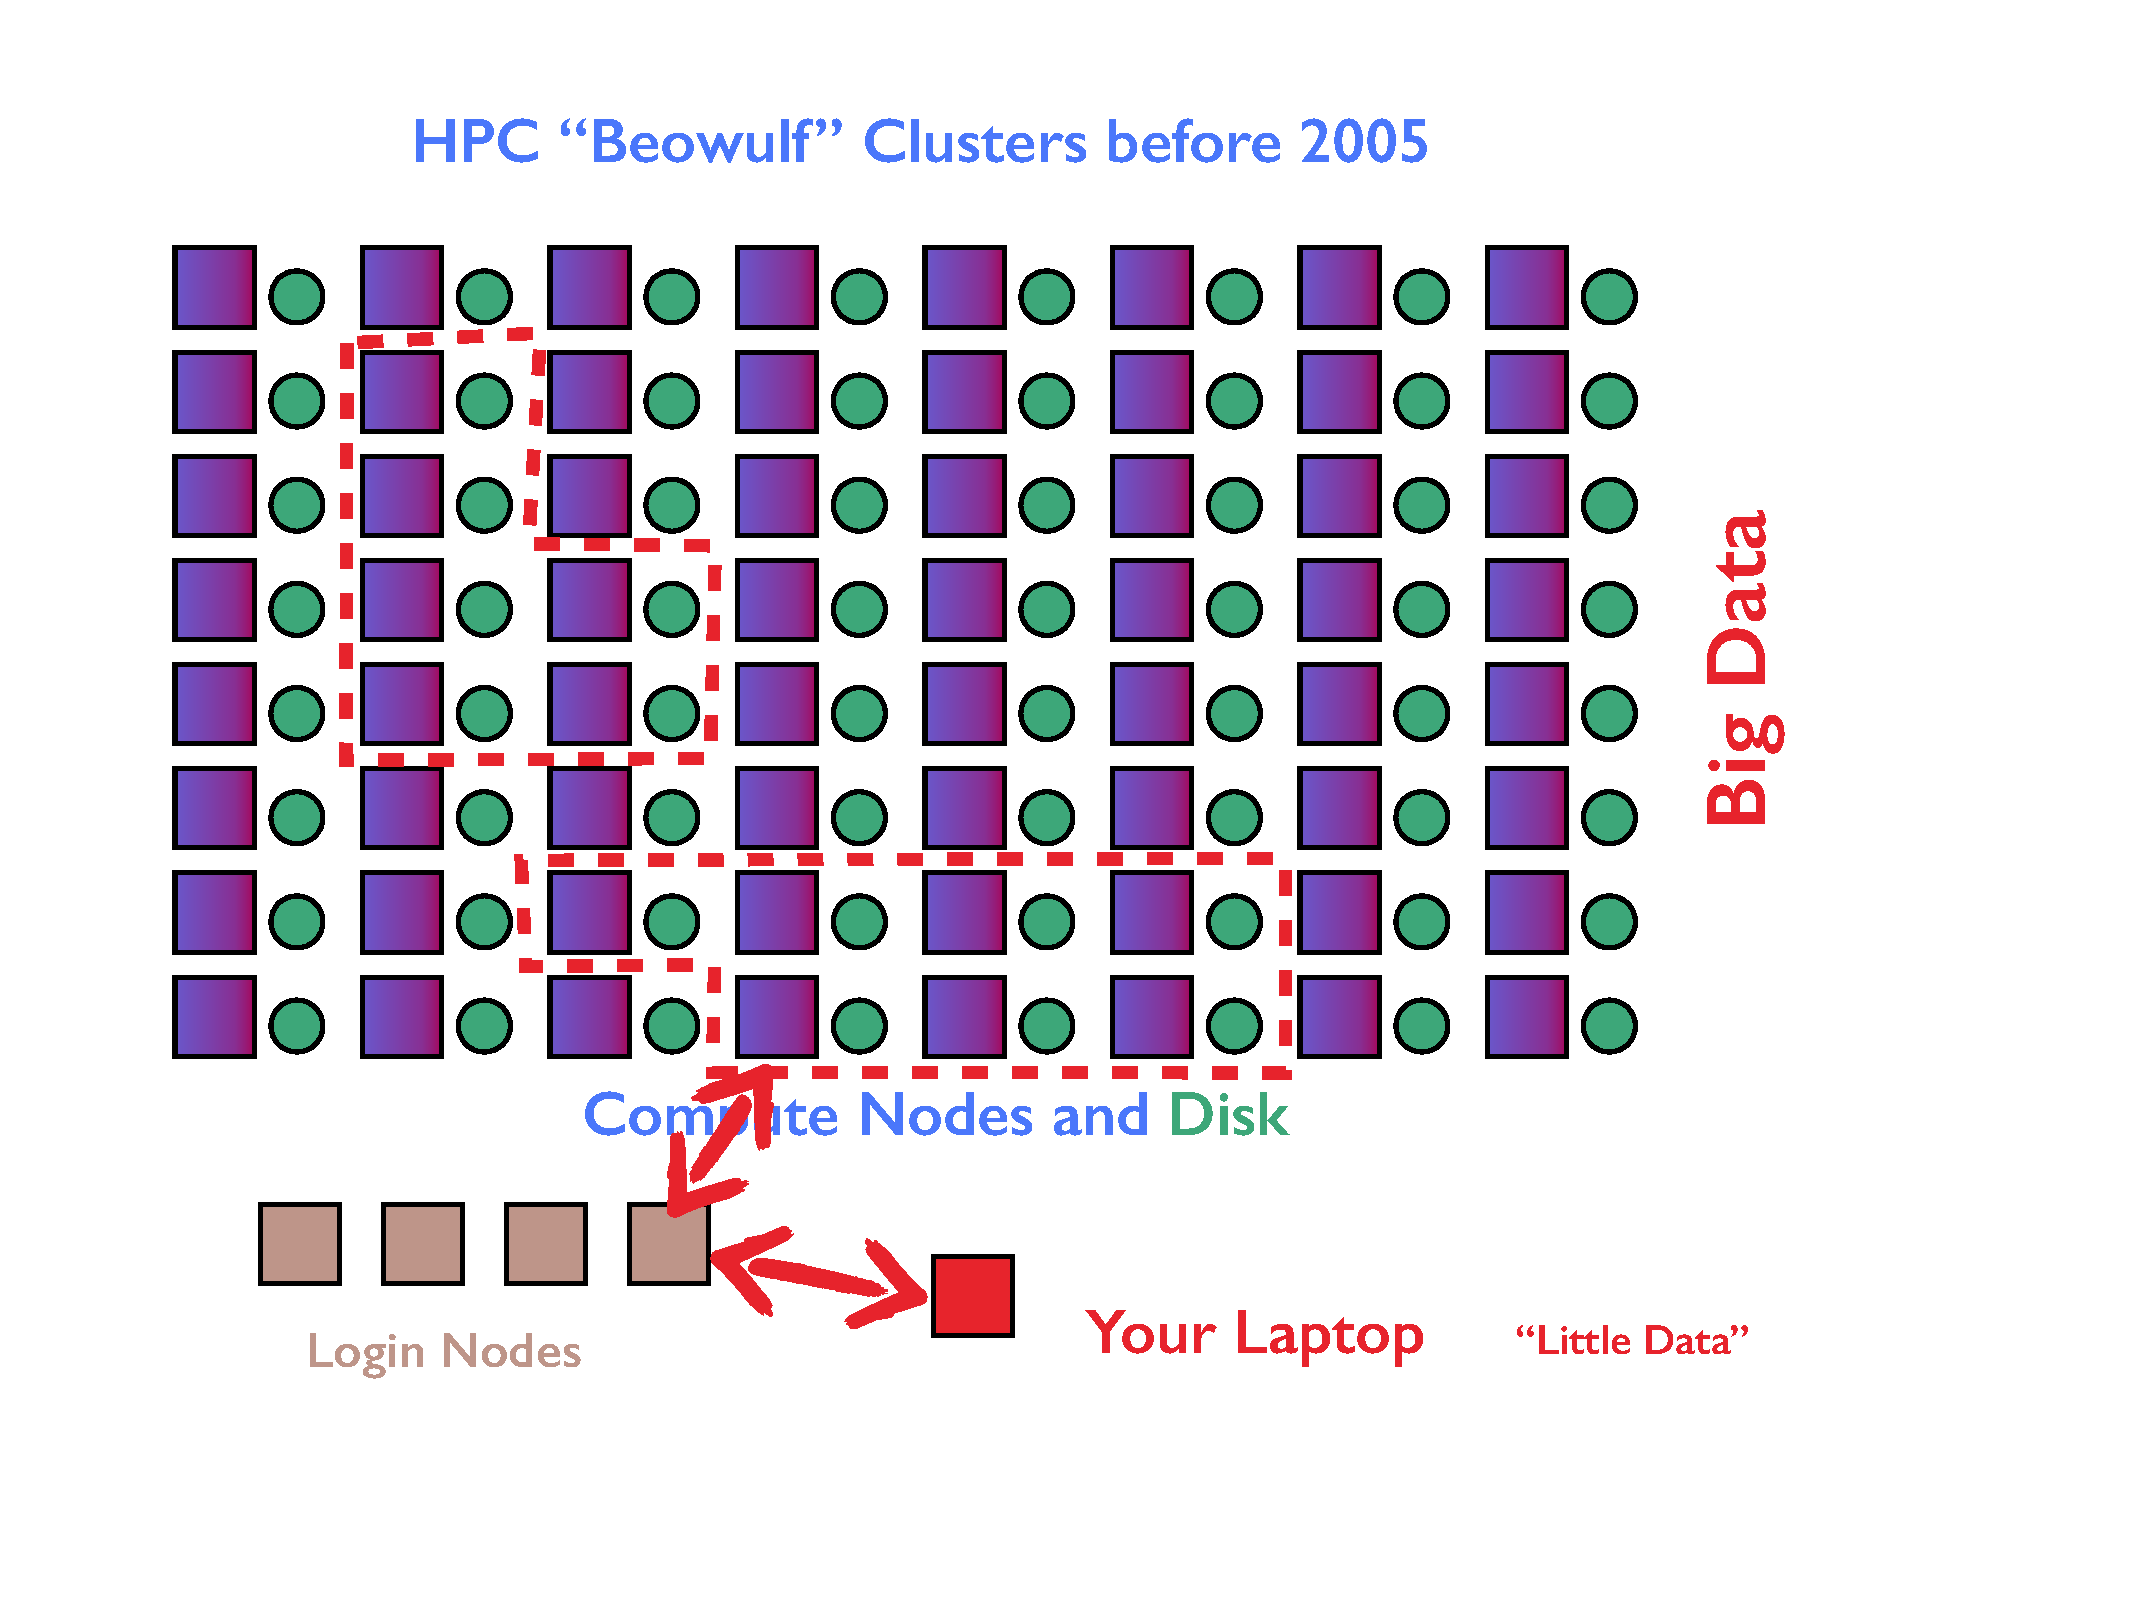
\includegraphics[width=0.95\textwidth]
{../common/pics/hardware/ParallelHardware22.pdf}
\end{frame}

\begin{frame}
  \begin{block}{Where to learn more?}
  \begin{itemize}
    \item \url{http://r-pbd.org/}
    \item \textbf{pbdDEMO} vignette
    \item \url{Google group: RBigDataProgramming}
  \end{itemize}
  \end{block}
\end{frame}

